\documentclass{scrartcl}

% Unterstützung für Deutsch
\usepackage[ngerman]{babel}
% Umterstützung für Bilder
\usepackage{graphicx}
% Pakete für die Darstellung und Eingabemöglichkeit von Umlauten
\usepackage[T1]{fontenc}
% Unterstützung für Quellcode
\usepackage{listings}
% Hyperlinks
\usepackage[colorlinks=true,linkcolor=black]{hyperref}
%Unterstützung für Unicode
\usepackage{ucs}
\usepackage[utf8x]{inputenc} 
%Unterstützung für Farbe
\usepackage{colortbl}

\usepackage{wrapfig}
\usepackage[bf]{caption2}

\usepackage{hhline}

\usepackage{amssymb}
\usepackage{fancyhdr}
\title{Graphicus}
\author{Paul Stahr, Yakup Ates}
\subtitle{Programm zur Darstellung von dreidimensionalen Graphen}


\lstset{language=Java, breaklines=true, basicstyle=\footnotesize}
\begin{document}
%%%%%%%%%%%%%%%%%%%%%%%%%%%%%%%%%%%%%%%%%%%%%%%%%% DECKBLATT ANFANG %%%%%%%%%%%%%%%%%%%%%%%%%%%%%%%%%%%%%%%%%%%%%%%%%%
\maketitle
\newpage

%%%%%%%%%%%%%%%%%%%%%%%%%%%%%%%%%%%%%%%%%%%%%%%%%% DECKBLATT ENDE %%%%%%%%%%%%%%%%%%%%%%%%%%%%%%%%%%%%%%%%%%%%%%%%%%
\tableofcontents
\newpage
%\section{Vorwort}
%\newpage
\section{Verwendete Software}
\subsection{OpenGl}
OpenGl (Open Graphics Library) ist eine Betriebssystem- und Programmiersprachenunabh"angige Schnittstelle, zur Entwicklung von 2D- und 3D- Computergrafik. Die erste Version wurde am 1. Juli 1992 ver"offentlicht. Zur Beschleunigung der Berechnung wird die Grafikkarte verwendet. Heutzutage gibt es viele Spiele, aber auch wissenschaftliche Programme die OpenGl zum Rendern ihrer Inhalte benutzen.
\subsection{Java}
Die erste Version der Programmiersprache Java ist im Jahr 1995 erschienen. Java ist eine Plattformunabh"angige, objektorientierte Programmiersprache. Mit einer passenden Laufzeitumgebung sind Programme in Java ohne "Anderung des Quellcodes auf jedem Betriebssystem lauff"ahig.
\subsection{LWJGL}
Trotz der Programmiersprachenunabh"angigkeit von OpenGl ist es dennoch n"otig eine Schnittstelle zwischen Java und OpenGl zu haben. LWJGL ist eine API die dies "ubernimmt. Es ist m"oglichst klein gehalten, und "ubertr"agt die Befehle, die zur Steuerung von OpenGl n"otig sind mit m"oglichst geringer Aufrufzeit in Java, sodass sie dort dann aufrufbar sind. Die offizielle Website ist  \url{http://lwjgl.org}.
\newpage
\section {Installation/Systemanforderungen}
Das Programm ben"otigt von sich aus keine Installation, es kann in jedes beliebige Verzeichnis oder auf jeden USB-Stick gezogen werden. Dennoch m"ussen bestimmte Voraussetzungen erf"ullt sein:
\begin{enumerate}
\item Das System muss OpenGl f"ahig sein. Andernfalls kann nur ein sehr geringer Teil des Programms genutzt werden.
\item Das System sollte "uber 512 MB Ram, 1Ghz CPU und 128 V-Ram verf"ugen.
\item Die Jave-Runtine-Environment muss mit mindestens Version 6 installiert sein. F"ur Windows gibt es allerdings eine Version, die ohne die java-jre auskommt.
\item Es sollte Schreibezugriff auf das Programm geben, da sonst keine Log-Dateien geschrieben werden k"onnen.
\end{enumerate}
\subsection{Windows}
Am sinnvollsten ist es die Standardversion des Programms unter Windows zu benutzen. Falls Sie jedoch keine JVM auf ihrem System haben, dann k"onnen sie die Windows Version benutzen, die komplett ohne weitere Software auskommt.
\subsection{Linux}
LWJGL muss auf dem System installiert sein. Das Programm ben\"otigt mindestens Version 1.7.2.
\subsubsection{LWJGL Installation}
Die Installation von LWJGL unterteilt sich in wenige Schritte. Sie m"ussen die Grundbefehle des Terminals benutzen k"onnen und eine Verbindung zum Internet haben.
\begin{enumerate}
 \item Laden Sie \emph{LWJGL} runter (z.B. unter \url{http://lwjgl.org}).
 \item Entpacken Sie die archivierte Datei und \"offne Sie den Entpackten Ordner.
 \item Wechseln sie in den Ordner ./lwjgl-[VERSIONSNUMMER]/native/linux.
 \item Kopieren Sie die Dateien die sich im Ordner ``linux'' befinden, in ihren /usr/lib Ordner. (Adminstratorrechte erforderlich)
 \item Sollte sich LWJGL noch in einem anderen lib-Ordner befinden l"oschen sie dieses. Folgende Dateien sind Teil von lwjgl:
\begin{tabbing}
\glqq libjinput-linux64.so\grqq   \= \glqq liblwjgl64.so\grqq   \= \glqq libopenal64.so\grqq \\
\glqq libjinput-linux.so\grqq \> \glqq liblwjgl.so\grqq \> \glqq libopenal.so\grqq 
\end{tabbing}
 \item Aktualisiere Sie die Liste der installierten Bibliotheken mit ``sudo ldconfig''.
\end{enumerate}
Falls keine Fehler aufgetreten sind, haben Sie nun \emph{LWJGL} erfolgreich installiert. 
\subsection{Aktivierung}
Nach erfolgreicher Installation "offnet sich beim Starten ein Fenster in dem sie gebeten werden, das Produkt zu aktivieren. Ohne Aktivierung sind speicher, lade und exportfunktionen nicht nutzbar. Die Aktivierung ist m"oglich indem sie eine E-mail an paul.stahr@gmx.de mit der angezeigten Id senden. Ihnen wird dann in den n"achsten Tagen ein Code zugeschickt, den sie in dieses Fenster eintragen k"onnen. Der Code Funktioniert nur f"ur das Entsprechende System. Selbstverst"andlich m"ussen sie die Software bei Updates nicht erneut Aktivieren, es sei denn dies wird explizit im Changelog erw"ahnt.
\newpage
\section{Das erste Projekt}
Dies ist eine Anleitung um einen einfachen Graphen zu zeichnen.\newline
Nach dem Start des Programmes sollte das Fenster in etwa so aussehen:\newline
\includegraphics[width=0.6\textwidth]{images/tutorial/interface1.png}
\begin{enumerate}
\item Gehen sie als erstes auf Extras und dort auf Optionen.
\end{enumerate}
\includegraphics[width=0.4\textwidth]{images/tutorial/options.png}
\begin{enumerate}
\item W"ahlen sie die Registrierkarte Licht/Umgebung.
\item Gehen sie auf Vorgabe W"ahlen und dort auf Bunt.
\item Wenn alles der Abbildung entspricht, dann k"onnen sie auf OK dr"ucken.
\end{enumerate}
\includegraphics[width=0.6\textwidth]{images/tutorial/interface2.png}
\begin{enumerate}
\item  Um einen Graphen hinzuzuf"ugen klicken sie auf den Plusbutton.
\end{enumerate}
\includegraphics[width=0.3\textwidth]{images/tutorial/graph.png}
\begin{enumerate}
\item W"ahlen sie als Typ 3D-Funktion
\item Die Ansicht stellen sie auf Fl"achen gegl"attet
\item Die Farbe stellen sie auf wei"s
\item Als Funktion geben sie \glqq \(x/y\)\grqq  ein.
\item Klicken sie auf OK
\end{enumerate}
\includegraphics[width=0.6\textwidth]{images/tutorial/interface3.png}\newline
Nun k"onnen sie mittels Rechts-, Linksklick und dem Mausrad die Perspektive im 3D-Fenster "andern. Wenn die Ansicht bei ihnen wie in der Abbildung aussieht, haben sie das Tutorial erfolgreich beendet.\newline
\newpage
\section{User Interface}
\subsection{Hauptfenster}
\includegraphics[width=0.7\textwidth]{images/program/main-window.png}\newline
Dies ist das Hauptfenster des Programms. Es unterteilt sich in vier Bereiche:\newline
1.Men"uleiste\newline
2.Toolmen"u\newline
3.Anzeigefenster f"ur Graphen\newline
4.Funktionen der aktuellen Graphen
\subsubsection{Men\"uleiste}
Die Men\"uleiste ist oben zu sehen, diese unterteilt sich in 3 teile, 'Datei', 'Ansicht', 'Bearbeiten' und 'Extras'.
Die Option 'Datei' unterteilt sich in in 7 weitere Optionen.
\begin{enumerate}
 \item Neu: Stellt alles wieder auf ``default'', somit werden aktuelle Graphen, Berechnungen etc. gel\"oscht. Das Programm ist bereit f\"ur ein neues Projekt.
 \item \"Offnen: Erm\"oglicht dem Benutzer gespeicherte Projekte wieder aufzurufen.
 \item Zuletzt ge\"offnet: Stellt die letzten 9 ge\"offneten Projekte dar.
 \item Speichern: Falls gerade mit einem bereits gespeichertem Projekt gearbeitet wird, kann hier die Datei mit den aktuellen Einstellungen \"uberschrieben werden, ohne eine neue Datei angeben zu m\"ussen.
 \item Speichern ... :Speichert das aktuelle Projekt an einem vom Benutzer ausgew\"ahlten Ort.
 \item Exportieren: Exportiert das Projekt, oder Teile davon in ein anderes Dateiformat.
 \item Beenden: Beendet das Programm.
\newpage
\end{enumerate}
In 'Ansicht' kann der Benutzer unter 3 Optionen w\"ahlen.
\begin{enumerate}
 \item Tools anzeigen: Erm\"oglicht das Ein-/Ausblenden der Leiste der linken Seite, der Benutzer bekommt somit ein gr\"o\ss{}eres Fenster f\"ur den Graphen.
 \item Graphenmen\"u anzeigen: Erm\"oglicht das Ein-/Ausblenden der Leiste der unteren Seite, wo die Funktionen aufgelistet werden. Der Benutzer bekommt so ein gr\"o\ss{}eres Fenster f\"ur den Graphen.
 \item Log anzeigen: Zeigt die Meldungen auf der Konsole, die f\"ur den Benutzer hilfreich sein k\"onnten, um m\"ogliche Fehler zu beheben.
\end{enumerate}
In 'Bearbeiten' kann der Benutzer unter 5 Optionen w\"ahlen.
\begin{enumerate}
 \item Kopieren: Noch nicht Implementiert
 \item Ausschneiden: Noch nicht Implementiert
 \item Einf\"ugen: Noch nicht Implementiert
 \item Projekteinstellungen: Erm\"oglicht das eintragen von Name, Autor und eine Beschreibung zum aktuellen Projekt. Siehe  \ref{chp:Projekt_Einstellungen_Fenster}.
\end{enumerate}
In 'Extras' kann der Benutzer unter 6 Optionen w\"ahlen.
\begin{enumerate}
 \item Hilfe: "Offnet diese \"uber das Programm, um Hilfe f\"ur den Benutzer zu gew\"ahrleisten.
 \item Zeichentabelle: Stellt 40 n\"utzliche Sonderzeichen dar, die man kopieren und im Programm verwenden kann. Siehe  \ref{chp:Zeichen_Fenster}.
 \item Auf updates pr\"ufen: Pr\"uft das Programm auf neuste Versionen, und stellt eine Liste der Verbesserungen von Version zu Version dar.Siehe  \ref{chp:Update_Fenster}.
 \item Einstellungen: Hier k\"onnen Einstellungen f\"ur das Programm getroffen werden.
 \item LWJGL-Lizenz: Hier wird die LWJGL-Lizenz dargestellt(Englisch).
 \item \"Uber ... : Hier sind die Bezeichnung des Programms, die Version und die Autoren des Programms aufgef\"uhrt. Siehe  \ref{chp:Info_Fenster}.
\end{enumerate}

\subsubsection{Toolmen\"u}
Das Toolmen\"u ist auf der linken Seite des Programms und unterteilt sich in viele Bereiche.
\begin{enumerate}
 \item Perspektive: Der Betrachtungswinkel zum Graphen kann hier gew\"ahlt werden.
 \item Slider: Hier k\"onnen Variablen deklariert und anhand eines Sliders auf einen Wert gesetzt werden.
 \item Variablen: Hier werden die deklarierten Variablen aufgelistet.
 \item Code Pad: Hier k\"onnen Berechnungen gemacht werden, es ist gleichzeitig eine Konsole und ein Taschenrechner. Um die Globalen Variablen in die Rechnungen mit einzubezeihen muss zus"atzlich zu Enter noch Shift gedr"uckt werden.
 \item Animation: Eine Variable wird hier pro Sekunde um einen gegebenen Wert erh\"oht, um Animationen mit Graphen zu erm\"oglichen.
\end{enumerate}

\subsubsection{Anzeigefenster der Graphen}
Hier werden die Graphen angezeigt, außerdem wenn erw"unscht Informationen "uber Framerate und Speicherauslastung. Die Steuerung der Perspektive ist mit Maus und Tastatur m"oglich:\newline
Maus:\newline
\begin{tabular}[b]{|l|l|}
\hline
Tasten &Funktion \\
\hline
links & dreht alles um die Kamera \\
\hline
rechts & dreht alles um den Nullpunkt \\
\hline
Mausrad & Bewegung nach vorne/hinten\\
\hline
\end{tabular}
\newline
Tastatur\newline
\begin{tabular}[b]{|l|l|}
\hline
Tasten &Funktion \\
\hline
Num links & Bewegung nach links \\
\hline
Num rechts & Bewegung nach rechts \\
\hline
Num oben & Bewegung nach oben \\
\hline
Num unten & Bewegung nach unten \\
\hline
Num plus & Bewegung nach vorne\\
\hline
Num minus & Bewegung nach hinten\\
\hline
Pfeil links & Drehung nach links\\
\hline
Pfeil rechts & Drehung nach rechts\\
\hline
Pfeil oben & Drehung nach unten\\
\hline
Pfeil unten & Drehung nach oben\\
\hline
\end{tabular}
\subsubsection{Liste der Graphen}
Hier wird der Graph mit dem vom Benutzer gew\"ahlten Einstellungen dargestellt, vorausgesetzt, dass das Graphenmen\"u unter 'Ansicht' nicht Ausgeblendet wurde. Es sind pro Graph 7 Symbole auf der linken Seite zu finden. Die Symbole werden von Links nach Rechts erkl\"art:
\begin{enumerate}
 \item Beim ersten Symbol kann die Farbe f\"ur die Funktion die als Graph dargestellt werden soll, ausgew\"ahlt werden.
 \item Beim zweiten Symbol von links gibt es 4 M\"oglichkeiten den Graphen darzustellen:
 \subitem \includegraphics[width=0.03\textwidth]{images/gIcons/dots.png} Punkte.
 \subitem \includegraphics[width=0.03\textwidth]{images/gIcons/lines.png} Linien.
 \subitem \includegraphics[width=0.03\textwidth]{images/gIcons/solid.png} Fl\"ache.(Nur bei 3D m\"oglich)
 \subitem \includegraphics[width=0.03\textwidth]{images/gIcons/smooth.png} Fl\"ache gegl\"attet. (Nur bei 3D m\"oglich)
 \item Ausgew\"ahlte Funktion Einblenden:\includegraphics[width=0.03\textwidth]{images/gIcons/visible.png} Ausblenden: \includegraphics[width=0.03\textwidth]{images/gIcons/invisible.png}
 \item Funktion wird berechnet: \includegraphics[width=0.03\textwidth]{images/gIcons/calculating.png} Funktion ist berechnet: \includegraphics[width=0.03\textwidth]{images/gIcons/not_calculating.png}
 \item Funktion nach oben verschieben: \includegraphics[width=0.03\textwidth]{images/gIcons/arrow_up.png} Funktion nach unten verschieben: \includegraphics[width=0.03\textwidth]{images/gIcons/arrow_down.png}
 \item Ausgew\"ahlte Funktion l\"oschen: \includegraphics[width=0.03\textwidth]{images/gIcons/delete.png}
\end{enumerate}
\subsection{Graphen}
\includegraphics[width=0.4\textwidth]{images/program/graph-window.png}\newline
Hier k"onnen die Einstellungen f"ur einen Graphen gemacht werden.
\subsubsection{Graphentypen}
\begin{tabular}[b]{|l|l|}
\hline
2D Funktion & Ordnet jedem x einen y zu. \\
\hline
2D Parametrisch & Ordnet jedem t einen x und y zu \\
\hline
2D Polar & Bildet die Funktion in einem Kreis ab \\
\hline
2D Plot & Macht zwei Listen als Plot sichtbar \\
\hline
3D Linie & Ordnet jedem t ein x, y und z zu \\
\hline
3D Funktion & Ordnet jedem x und y ein z zu \\
\hline
3D Parametrisch & Ordnet jedem u und v ein x, y und z zu \\
\hline
3D Polar & noch nicht implementiert \\
\hline
3D Plot & Macht drei Listen als Plot sichtbar \\
\hline
3D Kartesisch & Funktionen der Form x*a+y*b+z*c=d \\
\hline
\end{tabular}
\subsubsection{Transformationsmatrix}
Zur Transformation kann hier eine \(4 \cdot 4\) Matrix eingegeben werden. Die Funktion wird dann anhand dieser Matrix im homogenen Koordinatensystem transformiert.
\subsection{Zeichen}
\label{chp:Zeichen_Fenster}
\includegraphics[width=0.4\textwidth]{images/program/characters-window.png}\newline
Hier findet man alle Zeichen, die f"ur das Programm wichtig sind. Man kann sie bei bedarf mit dem Button \glqq Kopieren\grqq in die Zwischenablage legen.
\subsection{Optionen}
In den Optionen sind alle Einstellungen zu finden, die f"ur das Programm wichtig sind. Alles was hier eingestellt werden kann wird in der Options-datei gespeichert und ist somit auf dem gesamten System g"ultig.
\subsubsection{Bild}
\includegraphics[width=0.4\textwidth]{images/program/settings0-window.png}\newline
In diesem Fenster ist es m"oglich allgemeine Einstellungen zum Bild zu machen.
\subsubsection{Licht/Umgebung}
\includegraphics[width=0.4\textwidth]{images/program/settings1-window.png}\newline
Hier k"onnen die Einstellungen F"ur das Licht, oder eine CubeMap die von den Graphen gespiegelt wird, gemacht werden. Da die Berechnung von \newline
echtem Licht viel zu aufw"andig w"are vereinfacht man das Modell und teilt das Licht in drei Gruppen ein.\newline\newline
\begin{tabular}[ht]{|l|c|c|c|}
\hline
Lichtart & Abk"urzung & Effekt & Positionsabh"angig\\
Ambient & A & Grundlicht & Nein\\
Diffuse & D & Matte Reflektion & Lichtquelle zu Objekt\\
Specular & S & Glanzeffekte & Lichtquelle zu Objekt und Kamera\\
 \hline
\end{tabular}\newline\newline
Cubemaps sind 6 Bilder, die wie ein W"urfel um die Szene angeordnet werden. Diese Bilder k"onnen dann reflektiert werden. 
Dies ist zwar nicht mit dem sogenanten Raytracing zu vergleichen, da Graphen nicht sich selbst spiegeln k"onnen, es sorgt aber dennoch f"ur sehr sch\"one Effekte. Das Verzeichnis der Cubemap kann frei gew"ahlt werden. Eine Beispielmap befindet sich im Programmordner unter \glqq /data/cubemaps/1/\grqq .
\subsubsection{Erweitert}
\subsection{Projektinformationen}
\label{chp:Projekt_Einstellungen_Fenster}
\includegraphics[width=0.4\textwidth]{images/program/project-information-window.png}\newline
Hier k"onnen allgemeine Projektinformationen eingestellt werden.
\subsection{Update}
\label{chp:Update_Fenster}
\includegraphics[width=1\textwidth]{images/program/update-window.png}\newline
Hier wird die eigene, sowie die aktuelle Version des Programms angezeigt. Zus"atzlich kann man einsehen, was sich in den Versionen ge"andert hat. Damit das Changelog und die aktuelle Version angezeigt werden k"onnen, ist eine Verbindung zum Internet n"otig.
\subsection{Matrix Erstellen}
In diesem Fenster wird eine Erleichterung zum Erstellen von \(4 \cdot 4\) Matrizen kommen. Es ist jedoch noch nicht fertig implementiert.
\subsection{Log}
\label{chp:Log_Fenster}
\includegraphics[width=1\textwidth]{images/program/log-window.png}\newline
Im Log kann man eventuelle Fehler des Programms feststellen, oder einfach Informationen "uber das was getan wurde erhalten. Hier erscheinen allerdings nur Meldungen f"ur den Benutzer. Deutlich detailliertere Informationen erh"alt man in den Log-Dateien. Siehe ~\ref{chp:Log}.
\subsection{Info}
\label{chp:Info_Fenster}
\includegraphics[width=0.5\textwidth]{images/program/info-window.png}\newline
Im Informationsfenster kann man die Autoren und die Version des Programms sehen.
\newpage
\section{Datentypen}
\subsection{Integer}
Ein Integer ist eine Ganzzahl. Der Wertebereich den ein Integer umfassen kann liegt bei $-2^{63}$ bis $2^{63}-1$. Sollte dieser Bereich bei einer Berechnung "uberschritten werden wird die Berechnung mit Flie"skommazahlen durchgef"uhrt. Um einen Wert zu einer Ganzzahl zu konvertieren kann die Int-Funktion genutzt werden.
\subsection{Flie"skommazahl}
Bei einer Flie"skommazahl ist die Positions des Kommas nicht fest, es kann flie"sen. Das erm"oglicht es sehr gro"se aber auch sehr kleine Zahlen zu verarbeiten. Der Wertebereich liegt bei $-1.79769313486231570^{308}$ bis $1.79769313486231570^{308}$. Beim "uberschreiten dieses Bereiches wird die Zahl durch ein $\infty$ oder $NaN$ ersetzt. Bei Rechnungen mit einer Ganzzahl und einer Flie"skommazahl wird die Ganzzahl vor der Rechnung automatisch in eine Flie"skommazahl umgewandelt. Die Flie"skommazahl hat gegen"uber der Ganzzahl den Nachteil, dass sie immer nur etwa 15 Stellen-Genauigkeit besitzt. Um eine Zahl zu einer Flie"skommazahl zu konvertieren, kann die Float-Funktion genutzt werden.
\subsection{Zeichen}
Ein Zeichen ist dadurch gekennzeichnet, dass sich an jeder Seite ein ' befindet. In der Informatik ist jedem Zeichen ein Wert zugeordnet. Bei diesem Programm gelten die Zuordnungen aus dem unicode-Zeichensatz. Um eine Zahl zu dem zugeh"origen Zeichen zu konvertieren kann die char-Funktion verwendet werden.
\subsection{String}
Ein String ist eine Kette von Zeichen. Sie wird dadurch gekennzeichnet, dass sich an Anfang und Ende des Strings Anf"uhrungszeichen befinden. Es k"onnen alle Zeichen hineingeschrieben werden, au"ser Anf"uhrungszichen. Um eine Rechnung zu einem String zu konvertieren, kann die String-Funktion genutzt werden.
\subsection{Liste}
Eine Liste kann mehrere Objekte enthalten. Sie ist durch geschweifte Klammern gekennzeichnet. Eine verschachtelte Liste mit weiteren Listen in der Liste kann zus"atzlich als Matrix interpretiert werden. Bei Rechnungen mit Listen wirken sich die meisten Operationen so aus, dass die Zahl bzw. jedes Element der ersten Liste mit jedem Element der zweiten Liste verkn"upft wird, und daraus eine neue Liste entsteht. Die Liste ist das einzige Objekt, dass nicht immun gegen Ver"anderungen ist. Es k"onnen einzelne Werte ausgetauscht werden.

\newpage
\section{Wichtige Zeichen}
\subsection{Verkn"upfungen}
\begin{tabular}[ht]{|l|l|l|}
\hline
Zeichen & Name & R"uckgabetyp\\
\hline\hline
\unichar{"0022} &Anf"uhrungszeichen & \\ 
\unichar{"0025} &Modulo (\ref{chp:Modulo}) & Zahl\\ 
\unichar{"002A} & Multiplikation (\ref{chp:Multiplikation})& Zahl\\ 
\unichar{"002B} &Addition/Vorzeichen (\ref{chp:Addition}) & Zahl\\ 
\unichar{"002D} &Subtraktion/Vorzeichen  (\ref{chp:Subtraktion})& Zahl\\ 
\unichar{"002F} &Division (\ref{chp:Division})& Zahl\\ 
\unichar{"003C} &Kleiner (\ref{chp:Kleiner})& Wahrheitswert\\ 
\unichar{"003D} &Gleich (\ref{chp:Gleich})& Wahrheitswert\\ 
\unichar{"003E} &Gr"o"ser (\ref{chp:Gr"o"ser})& Wahrheitswert\\ 
\unichar{"005E} &Expon & Zahl\\ 
\unichar{"00AC} & Nicht (\ref{chp:Nicht})& Wahrheitswert/Ganzzahl\\
\(\curlywedge\) & Und (\ref{chp:Und})&  Wahrheitswert/Ganzzahl \\
 \(\curlyvee\) & Oder (\ref{chp:Oder})&  Wahrheitswert/Ganzzahl\\
\unichar{"2022} & Multiplikation f"ur Matrizen  (\ref{chp:Matrizenmultiplikation})& Matrix \\
\unichar{"2192} & Zuweisung & Rechnung\\
\unichar{"2208} & Element aus (\ref{chp:Element_aus})& Wahrheitswert \\
\unichar{"2209} & Nicht Element aus (\ref{chp:Nicht_Element_aus})& Wahrheitswert \\
\unichar{"2260} & Ungleich (\ref{chp:Ungleich})& Wahrheitswert \\
\unichar{"2264} & Kleiner gleich (\ref{chp:Kleiner_gleich})& Wahrheitswert \\
\unichar{"2265} & Gr"o"ser gleich  (\ref{chp:Gr"o"ser_gleich})& Wahrheitswert \\
\unichar{"2286} & Teilmenge aus  (\ref{chp:Teilmenge_aus})& Wahrheitswert \\
\unichar{"2288} & Nicht Teilmenge aus (\ref{chp:Nicht_Teilmenge_aus}) & Wahrheitswert \\
\(\circ\) &Vereinigung & String \\
\(\times\) &Kreuzprodukt  & Matrix \\ 
\hline
\end{tabular}

\subsection{Mengen}
\begin{tabular}[ht]{|l|l|}
\hline
Zeichen & Name\\
\hline\hline
\(\mathbb{C}\) & Komplexe Zahlen \\
\(\mathbb{N}\) & Nat"urliche Zahlen \\
\(\mathbb{P}\) & Primzahlen \\
\(\mathbb{Q}\) & Rationale Zahlen \\
\(\mathbb{R}\) & Reelle Zahlen \\
\(\mathbb{Z}\) & Ganze Zahlen \\
\hline
\end{tabular}
\subsection{Zahlen}
\begin{tabular}[ht]{|l|l|}
\hline
Zeichen & Name\\
\hline\hline
\unichar{"221E} & Unendlich\\
\(\pi\) & Konstante Kreiszahl Pi\\
$e$ & Eulersche Konstante\\
$ i $ & Imagin"are Zahl\\
\hline
\end{tabular}
\newpage
\section{Funktionen und Rechenoperationen}
\subsection{Grundrechenarten}
Grunds"atzlich gilt bei allen Rechenarten, dass wenn zwei Ganzzahlen verkn"upft werden, das Ergebinis wenn m"oglich ebenfalls eine Ganzzahl ist. Sollte die Rechnung jedoch eine Kommazahl oder eine Zahl die den Wertebereich der Ganzzahlen "uber oder unterschreitet ergeben, so wird eine Flie"skommazahl zur"uckgegeben. Au"serdem werden Berechnungen beliebig umgestellt um schon m"oglichst viel zu Berechnen. Beispielsweise ergibt \(2*(b/3)=0.6666666666666666*b\), wenn die Variablen erst sp"ater eingegeben werden.
\subsubsection{Addition}
\label{chp:Addition}
Mit dem Zeichen \glqq +\grqq  k"onnen zwei Zahlen addiert werden.
\subsubsection{Subtraktion}
\label{chp:Subtraktion}
Mit dem Zeichen \glqq -\grqq  k"onnen zwei Zahlen subtrahiert werden.
\subsubsection{Multiplikation}
\label{chp:Multiplikation}
Mit dem Zeichen \glqq *\grqq  k"onnen zwei Zahlen miteinander multipliziert werden.
\subsubsection{Matrizenmultiplikation}
\label{chp:Matrizenmultiplikation}
Da bei einer normalen Multiplikation Matrizen als Listen gewertet werden, gibt es ein Zeichen, dass extra daf"ur ist Matrizen zu Multiplizieren. Dieses Zeichen ist: \glqq \unichar{"2022}\grqq.
\subsubsection{Kreuzprodukt}
Das Kreuzprodukt l"asst sich auf zwei Vektoren anwenden. Eine Matrix ist dann ein Vektor, wenn sie nur eine Spalte besitzt. Das Ergebnis ist ebenfalls ein Vektor.
\subsubsection{Skalarprodukt}
Das Skalarprodukt zweier Vektoren l"asst sich mit dem Zeichen \glqq \(\ast\)\grqq berechnen.
\subsubsection{Division}
\label{chp:Division}
Mit dem Zeichen \glqq /\grqq  wird eine Zahl durch eine andere geteilt.
\subsubsection{Modulo}
\label{chp:Modulo}
Modulo ist der Rest der bei einer Division auftritt, wenn das Ergebnis eine Ganzzahl sein soll. Die Besonderheit hier ist, dass wenn eine der beiden Zahlen negativ ist, das damit auch das Ergebnis ein negatives ist.
\subsection{Konvertierungen}
\subsubsection{Integer}
\includegraphics[width=0.7\textwidth]{images/functions/integer.png}\newline
Die Funktion int() kann genutzt werden um aus einer Flie"skommazahl, einem Zeichen oder String eine Ganzzahl zu erzeugen. Die Nachkommastellen werden bei einem Flie"skommawert einfach abgeschnitten. Will man das nicht haben, kann man die Funktionen round(a) (siehe \ref{chp:Gr"o"ser_gleich}) und int(a) kombinieren. Beispielsweise ist int(round(1.6)) = 2 w"ahrend int(1.6) = 1 ist.
\subsubsection{Float}
Die Funktion float(a) kann genutzt aus werden um aus einer Ganzzahl, Zeichen oder Zeichenkette eine Flie"skommazahl zu erzeugen.
\subsubsection{Char}
Die Funktion char(a) erzeugt aus einer Zahl das ihm in Unicode zugeordnete Zeichen. Der Aufruf char(65) ergibt beispielsweise 'A'.
\subsubsection{Zeichenkette}
Die Funktion string(a) erzeugt aus einer Rechnung einen String. Die Rechnung selbst wird abei nicht ver"andert.
\subsubsection{Compile}
Die Funktion compile(a) kann genutzt werden, um aus einem String wieder eine Rechnung zu erhalten.
\subsubsection{Char zu Zeichenkette}
Hat man eine Liste aus Zeichen und will diese zu einem String konvertieren, kann man die Funktion chartostring(a) nutzen.
\subsubsection{Format}
Mit der Funktion format(a,b) ist es m"oglich eine Rechnung zu einer Zeichenkette f"ur andere Programme zu konvertieren. Die Variable b ist die Rechnung und a definiert durch eine Zeichenkette das gew"unschte Programm. Es sind folgende Ausgaben m"oglich:
\begin{itemize}
\item \grqq calgraph\grqq :Standartausgabe des Programmes
\item \grqq latex\grqq :Ausgabe f"ur latex-Formeln
\item \grqq open\_office\grqq :Ausgabe f"ur Open-Office-Formeleditor
\end{itemize}
\subsection{Zufall}
\subsubsection{Zufallszahl}
Zufallszahlen k"onnen mit der Funktion rand() erzeugt werden, wie eine Zahl zwischen 0 und 1 zur"uck gibt.
\subsubsection{Liste mit Zufallszahlen}
Eine Liste mit Zufallszahlen kann durch die Funktion randlist(x) erzeugt werden.
\subsubsection{Matrix mit Zufallszahlen}
Eine Matrix mit Zufallszahlen kann durch die Funktion randmat(x,y) erzeugt werden.
\subsection{Bin"ar}
\subsubsection{Nicht}
\label{chp:Nicht}
Kehrt den Wahrheitswert um.
\subsubsection{Und}
\label{chp:Und}
Diese Funktion kann auf Wahrheitswerte sowie Ganzzahlen angewendet werden. Das Ergebnis der Operation kann an folgender Wahrheitstabelle abgelesen werden.\newline
\begin{tabular}[b]{|l|l|l|}\hline
 &  true & false \\\hline
true & true & false \\\hline
false & false & false \\\hline
\end{tabular}
\subsubsection{Oder}
\label{chp:Oder}
Diese Funktion kann auf Wahrheitswerte sowie Ganzzahlen angewendet werden. Das Ergebnis der Operation kann an folgender Wahrheitstabelle abgelesen werden.\newline
\begin{tabular}[b]{|l|l|l|}\hline
 &  true & false \\\hline
true & true & true \\\hline
false & true & false \\\hline
\end{tabular}
\subsubsection{Gleich}
\label{chp:Gleich}
Pr"uft ob zwei Zahlen oder Wahrheitswerte gleich sind und gibt true oder false zur"uck.
\subsubsection{Ungleich}
\label{chp:Ungleich}
Pr"uft ob zwei Zahlen oder Wahrheitswerte ungleich sind und gibt true oder false zur"uck.
\subsubsection{Kleiner}
\label{chp:Kleiner}
Die Verkn"upfung \unichar{"003C} pr"uft ob eine Zahl kleiner ist als eine andere.
\subsubsection{Gr"o"ser}
\label{chp:Gr"o"ser}
Die Verkn"upfung \unichar{"003D} pr"uft ob eine Zahl gr"o"ser ist als eine andere.
\subsubsection{Kleiner gleich}
\label{chp:Kleiner_gleich}
Die Verkn"upfung \unichar{"2264} pr"uft ob eine Zahl kleiner oder gleich einer anderen ist.
\subsubsection{Gr"o"ser gleich}
\label{chp:Gr"o"ser_gleich}
Die Verkn"upfung \unichar{"2265} pr"uft ob eine Zahl gr"o"ser oder gleich einer anderen ist.
\subsubsection{Element aus}
\label{chp:Element_aus}
Die Verkn"upfung \unichar{"2208} pr"uft ob etwas ein Element aus einer Menge oder Liste ist.
\subsubsection{Nicht Element aus}
\label{chp:Nicht_Element_aus}
Die Verkn"upfung \unichar{"2209} pr"uft ob etwas nicht ein Element aus einer Menge oder Liste ist.
\subsubsection{Teilmenge aus}
\label{chp:Teilmenge_aus}
Die Verkn"upfung \unichar{"2286} pr"uft ob eine Menge die Teilmenge einer anderen ist.
\subsubsection{Nicht Teilmenge aus}
\label{chp:Nicht_Teilmenge_aus}
Die Verkn"upfung \unichar{"2288} pr"uft ob eine Menge nicht die Teilmenge einer anderen ist.
\subsection{Vereinigung}
\label{Vereinigung}
Die Vereinigung kann genutzt werden um aus zwei Strings einen zu machen. Der Fachbegriff f"ur diese Operation lautet Konkatenation.
\subsection{System}
\subsubsection{Garbage Collector}
Durch die Funktion gc kann der \glqq Garbage Collector\grqq  von Java aufgerufen werden. Dadurch werden nicht mehr ben"otigte Ressourcen wieder freigegeben. Es gibt jedoch keine Garantie, dass der Garbage Collector wirklich aufgerufen wird. Gibt immer true zur"uck.
\subsubsection{Speichern}
Die Funktion save() Speichert das Projekt auf das aktuell ge"offnete. Gibt true zur"uck wenn es erfolgreich war und false wenn nicht.
\subsubsection{Lesen}
Mit der Funktion read(a) k"onnen Bilder oder Textdateien in das Programm gelesen werden. Bilder werden dadurch zu einer zweidimensionalen Liste, Textdateien zu einer Zeichenkette. Die Variable muss eine Zeichenkette mit dem dateipfad entsprechen.
\subsubsection{Schreiben}
Mit der Funktion write(a, b) kann eine Zeichenkette in eine Datei geschrieben werden. Dabei muss a eine Zeichenkette sein, die den Speicherort definiert und b muss die Zeichenkette sein, die geschrieben werden soll.
\subsection{Runden}
\label{chp:Runden}
Die Funktion round(a) kann eine Zahl runden. Wird ihr ein Flie"skommawert "ubergeben, so ist der resultierende Wert ebenfalls vom Typ Flie"skommazahl sein.\newline
\includegraphics[width=0.7\textwidth]{images/functions/round.png}
\subsection{Maximum}
\subsubsection{Maximum von zwei Zahlen}
Die Funktion max(a,b) gibt den Wert zur"uck, der gr"o"ser ist.
\subsubsection{Maximum aus einer Liste}
Die Funktion max(a) muss mit einer Liste aufgerufen werden und gibt daraus den Gr"o"sten Wert zur"uck.
\subsection{Minimum}
\subsubsection{Minimum von zwei Zahlen}
Die Funktion min(a,b) gibt den Wert zur"uck, der kleiner ist.
\subsubsection{Minimum aus einer Liste}
Die Funktion min(a) muss mit einer Liste aufgerufen werden und gibt daraus den kleinsten Wert zur"uck.
\subsection{Absolut}
Die Funktion abs() macht aus einer Zahl eine Positive.\newline
\includegraphics[width=0.7\textwidth]{images/functions/absolute.png}
\subsection{Kardinalit"at}
Mit der Funktion kard(a) kann die Kardinalit"at, oder auch Anzahl der Elemente einer Liste ermittelt werden.
\subsection{Gr"o"ster gemeinsamer Teiler}
Die  Funktion ggt(a,b) berechnet den gr"o"sten gemeinsamen Teiler aus zwei Zahlen. Das Ergebnis ist auch bei negativen Eingabewerten positiv. Die Methode sieht folgenderma"sen aus:\newline
\begin{minipage}{\textwidth}
\begin{lstlisting}
public static final long ggt (long a, long b){
   if (a < 0)
      a = -a;
   if (b < 0)
      b = -b;
   while ((a%=b)!=0)
      if ((b%=a)==0)
         return a;
   return b;
}
\end{lstlisting}
\end{minipage}
\subsection {Kleinstes gemeinsames Vielfaches}
Die Funktion kgv(a,b) berechnet das kleinste gemeinsame Vielfache zweier Zahlen. Sollte das Ergebnis nicht in den Bereich der Ganzzahlen passen, so wird -1 zur"uckgegeben. Au\ss{}erdem ist das Ergebnis immer positiv, auch wenn die Eingabe negativ war. Die Methode sieht folgenderma"sen aus:\newline
\begin{minipage}{\textwidth}
\begin{lstlisting}
public static final long kgv (long a, long b){
   if (a < 0)
      a = -a;
    if (b < 0)
      b = -b;
   final long c = a / ggt(a,b);
   final long kgv = c * b;
   return kgv / b == c ? kgv : -1;
}
\end{lstlisting}
\end{minipage}
\subsection{Kombinatorik}
\subsubsection{Anzahl der Permutationen}
Die Funktion um die Anzahl der Permutationen zu berechnen lautet npr(a,b). Die Methode, die hinter der Berechnung steckt ist folgende:\newline
\begin{minipage}{\textwidth}
\begin{lstlisting}     
public static final long npr(long n, long k){
   if (n < 0 || k < 0 || n < k)
      return -2;
   if (n < fakCacheLong.length)
      return fakCacheLong[(int)n]/fakCacheLong[(int)(n-k)];
   if (n<(k<<1))
      k = n-k;
   long erg = 1;
   for (long i=k;i<n;i++)
      if (erg != (erg *= i)/i)
         return -1;
   return erg;
}
\end{lstlisting} 
\end{minipage}
\subsubsection{Anzahl der Kombinationen}
Der Binomialkoeffizient ist eine Mathematische Funktion, um kombinatorische Aufgaben zu l\"osen. Die Methode hei\ss{}t  ncr(n, k), wobei n und k als 
Ganzzahlen interpretiert werden. Bei zu gro"sen Werten ist der R"uckgabewert -1 und bei ung"ultigen Eingabeparametern -2. Folgende Mathematische Formel steckt hinter der Funktion.\newline
 $ {n \choose k} = \frac {n!} {k! \cdot (n-k)!}  $\newline Dennoch sieht unserer Methode etwas anders aus:\newline
\begin{minipage}{\textwidth}
\begin{lstlisting}     
public static final long ncr (final long n, long k){
   if (k > n || k < 0 || n < 0)
      return -2;
   if (n < fakCacheLong.length)
      return fakCacheLong[(int)n]/(fakCacheLong[(int)k]*fakCacheLong[(int)(n-k)]);
   if (n<(k<<1))
      k = n-k;
   long erg = 1;
   final long nk = n-k;
   for (int i=1;i<=k;i++)
      if ((erg /= i) != (erg *= nk + i) / (nk + i))
         return -1;
   return erg;
}
\end{lstlisting} 
\end{minipage}
Die Methode l"asst sich in 4 Teile unterteilen: 
\begin{enumerate}  
\item "Uberpr"ufen ob falsche nicht l"osbare Eingaben gemacht wurden.  
\item Das Ergebnis wenn m"oglich auf schnelle Weise durch bereits berechnete Fakult"aten berechnen.  
\item ncr(n,n-k) statt ncr(n,k) berechnen, falls \(n<k \cdot 2\), da  das Ergebnis das gleiche ist, aber das neue k kleiner, also Effizienter.  
\item Durch eine Schleife den ncr berechnen. Danach das Ergebnis ausgeben, oder wenn w"ahrend der Berechnung ein "Uberlauf auftritt -1. 
\end{enumerate}.
\subsection{If Abrage}
Mit der Funktion ifn(a,b,c) k"onnen Abfragen realisiert werden. Sollte die Berechnung in a true ergeben wird b zur"uckgegeben, bei false c.
\subsection{Abfrage von Benutzereingabe}
Mit der Funktion request(a) kann man den Benutzer dazu auffordern eine Eingabe zu machen. Der Parameter a muss eine Zeichenkette sein und der R"uckgabewert ist ebenfalls immer eine Zeichenkette. Die Methode pausiert die Berechnung so lange, bis eine Eingabe gemacht wurde. Es ist auch m"oglich mit request(a,b) durch b ein timeout in Sekunden anzugeben, nach dem sich das Fenster automatisch schlie"st.
\subsection{Warten}
Mit der Funktion sleep(a), kann eine Zeit gewartet werden. Die Zeit wird dabei in Sekunden abgegeben.
\subsection{Wurzel}
\subsubsection{Quadrat Wurzel}
\includegraphics[width=0.7\textwidth]{images/functions/wurzel.png}\newline

Hier werde ich den so genannten \glqq sqrt\grqq Algorithmus erl"autern. Es handelt sich n"amlich um die Berechnung der quadratischen Wurzel von dem gegebenen Parameter x.\newline

Im Mathematischen Sinne kann man die Wurzel mit einem N"aherungsverfahren, und zwar dem Newton-Verfahren.\newline
Wie bereits erw"ahnt ist es ein N"aherungsverfahren, welches genauer wird je "ofter man es iteriert.\newline
Sei \(x\) gegeben, wobei \(x\unichar{"2208} | x > = 0\), und \(y\) das daraus berechnete Ergebnis, wobei \(y \unichar{"2208}\) .\newline

Die Gleichung :
\begin{displaymath}
\frac{(2-1)\cdot y^n+x }{ 2 \cdot y^{n-1} } \qquad
\end{displaymath}
 entspricht dem Newton-Verfahren, diese haben wir jedoch etwas angepasst, um unn"otige Rechenoperationen zu vermeiden.
Es resultierte :\newline 

\begin{displaymath}
\frac{ y \cdot y + x}{2 \cdot y } \qquad
\end{displaymath}

Au"serdem haben wir ausgeschlossen, dass \(x < 0\) ist, und wenn \(x = 0\), dann ergibt es ohne eine Berechnung 0.\newline
Sehen wir uns den Algorithmus mal an.\newline
\begin{minipage}{\textwidth}
\begin{lstlisting}
public static final double sqrt(final double n){
   if(n<0)
      return Double.NaN;
   if(n==0)
      return 0;
   double erg=n;
   for(int i=1;i!=11;i++)
      erg=(erg*erg+n)/(2*erg);
   return erg;        
}
\end{lstlisting}
\end{minipage}

An dem Algorithmus wird die oben genannte Gleichung sehr sch"on und eindeutig deutlich. Wir iterieren die Gleichung 10-mal, da uns bereits die Genauigkeit des Ergebnisses nach 10 Schritten gen"ugte. Da der Algorithmus nicht besonders schwer ist, werde ich ihn nicht detailliert durchgehen. Was m"oglicherweise jedoch nicht klar ist, ist das \glqq Double.NaN\grqq, NaN steht f"ur Not a Number, aus dem Algorithmus geht also hervor das wenn die Wurzel von x berechnet werden soll, x jedoch kleiner als 0 ist, so ist es nicht definiert und man bekommt NaN ausgegeben.\newline
\subsubsection{N-te Wurzel}
Auch haben wir einen Algorithmus zum Berechnen der n-ten Wurzel von x. Die oben genannte Gleichung ist hier unver"andert und das Verfahren dementsprechend identisch:

\begin{displaymath}
\frac{(2-1) \cdot y^n+x}{2 \cdot y^{(n-1)}} \qquad
\end{displaymath}

Da wir die Gleichung jedoch nicht ver"andert haben, ist der Algorithmus etwas anders.\newline
\begin{minipage}{\textwidth}
\begin{lstlisting}
public static double rt(double y, int n){
   if(n<=0)
      return Double.NaN;
   if(y==0)
      return 0;
   double erg=y;
   for(int i=1;i!=200;i++)
      erg=((n-1)*pow(erg,n)+y)/(n*pow(erg,n-1));
   return erg;
}
\end{lstlisting}
\end{minipage}

Auch hier kommt die genannte Gleichung sehr gut zum Vorschein. Der Parameter n ist hier die Potenz der Funktion und y die zu berechnende Zahl. Die hier genutzte Methode pow(x, exponent) ist ebenfalls von uns geschrieben und berechnet eine Potenz von x mit dem Exponenten exponent. Ich komme sp"ater auf diese Methode zur"uck, um sie etwas weiter zu erl"autern. Die Iteration haben wir provisorisch auf 199 gesetzt, um eine genaue grenze zu ermitteln m"ussten wir eine ausführliche und Zeitaufwendige Statistik f"uhren, belassen wir es vorerst auf 199.\newline
Falls nicht klar ist, was mit der Iteration 199 gemeint ist: Das hei"st, das die oben aufgef"uhrte Funktion 199-mal wiederholt wird, um dementsprechend sehr genaue Ergebnisse zu ermitteln, da wie bereits erw"ahnt \glqq je \grqq ofter man iteriert, desto genauer wird das Ergebnis\grqq .\newline
\subsubsection{W"urfel}
\includegraphics[width=0.7\textwidth]{images/functions/cube_wurzel.png}\newline
Die 3-te Wurzel auch Würfel-Wurzel genannt kann durch die Funktion cbrt() gezogen werden.
\subsection{Potenz}
Die pow(x, exponent) Methode haben wir bereits bei der Berechnung der n-ten Wurzel von x gesehen, was aber ist die pow Methode und was macht sie?
Die pow(x, exponent) Methode berechnet die Potenzen einer Zahl x. Beispielsweise wenn wir als x 2 eingeben und als Exponent 2, so wird er uns die 4 ausgeben, da \(2^2 = 4\).
Um unser Beispiel weiter zu analysieren: \(2^2 == 4\), der Exponent beschreibt also die Anzahl, der Zahl x, welche mit sich selbst multipliziert wird, wenn wir also 2 haben, rechnen wir , die Zahl 2 erscheint zwei mal, da der Exponent 2 ist. Sehen wir uns den Algorithmus an.
\begin{minipage}{\textwidth}
\begin{lstlisting}
public static Number pow (long x, long exponent){
  if (exponent<0)
    return Math.pow(x, exponent);
  if(exponent==0)
    return 1;
  BigInteger erg = BigInteger.valueOf(x);
  while (exponent != 1){
    erg = (exponent&1)==0 ? erg.multiply(erg) : erg.multiply(erg).multiply(BigInteger.valueOf(x));
    exponent >>= 1;
  }
  return erg;
}
\end{lstlisting}
\end{minipage}
Um Syntax Fragen direkt zu kl"aren: \(a >>= 1\) hei"st, \(a = a/2\) , und man sieht das erg den Typ BigInterger hat, BigInterger kann sehr gro"se Zahlen beinhalten, jedoch muss man Methoden f"ur Rechenoperationen benutzen, in dieser Methode sieht man die Multiplikation also multiply(erg). Also wird hier entweder erg mit sich selbst multipliziert, oder mit x. Exponent\&1 hei"st so viel wie Exponent modulo 2.
\subsection{Trigonometrisch}
\subsubsection{Sinus}
\includegraphics[width=0.7\textwidth]{images/functions/sinus.png}\newline
Die Sinusfunktion kann durch sin(a) berechnet werden. Die Berechnung erfolgt im Bogenma"s.
\subsubsection{Cosinus}
\includegraphics[width=0.7\textwidth]{images/functions/cosinus.png}\newline
Die Cosinusfunktion kann durch cos(a) berechnet werden. Die Berechnung erfolgt im Bogenma"s.
\subsubsection{Tangens}
Die Tangensfunktion kann durch tan(a) berechnet werden. Die Berechnung erfolgt im Bogenma"s.
\subsubsection{Hyperbolischer Sinus}
\includegraphics[width=0.4\textwidth]{images/functions/hyperbolic_sinus.png}\newline
Der Hyperbolische Sinus kann mit der Funktion sinh(a) berechnet werden.
\subsubsection{Hyperbolischer Cosinus}
\includegraphics[width=0.4\textwidth]{images/functions/hyperbolic_cosinus.png}\newline
Der Hyperbolische Cosinus kann mit cos(a) berechnet werden.
\subsubsection{Hyperbolischer Tangens}
\includegraphics[width=0.4\textwidth]{images/functions/hyperbolic_tangens.png}\newline
Der Hyperbolische Tangens kann mit der Funktion tanh(a) berechnet werden.
\subsection{Variablen}
\subsubsection{Definiere}
Mit der Funktion define(a) kann eine Variable mit dem Namen a definiert werden. Eine neue Variable enth"alt nach der Definition einen Nullzeiger.
\subsubsection{Zuweisung}
Die Zuweisung ist dazu da um Variablen Werte zuzuweisen. Das Zeichen f"ur die Zuweisung ist \(b \unichar{"2192} a\), es kann aber auch die Funktion \(set(a,b)\) genutzt werden. Dabei ist a die Variable der der Wert b zugewiesen werden Soll. Es ist auch m"oglich eine Listenstelle einen Wert zuzuweisen. Wenn man beispielsweise \(5 \unichar{"2192} a[2]\) schreibt und \(a = \{1,2,3\}\) war, dann ist danach \(a = \{1,2,5\}\). Wird eine Variable in der ein Liste gespeichert ist, einer anderen zugewiesen, so wird die Liste kopiert, was aus Performancegr"unden ber"ucksichtigt werden sollte.
\subsubsection{L"osche}
Mit der Funktion delete(a) kann eine Variable wieder gel"oscht werden.
\subsection{L"ose}
Die Funktion solve(a,b) kann zum Aufl"osen einfacher Gleichungen benutzt werden. Dabei ist a die Gleichung und b die Variable, nach der aufgel"ost werden soll.
\newpage
\section{Interessante/Formsch"one Graphen}
\subsection{Zwei Wellen}
\begin{tabular}[b]{|c|c|}\hline
\rowcolor[gray]{0.5}
Art & 3D Funktion \\
\rowcolor[gray]{1}
f(x,y) & \(\left (\frac{\sin\left(a \cdot \sqrt{(x-10)²+y²}+c\right)}{\sqrt{(x-10)²+y²+0.5}}+\frac{\sin\left(a \cdot \sqrt{(x+10)²+y²}+c\right)}{\sqrt{(x+10)²+y²+0.5}}\right )\cdot b\)\\
\rowcolor[gray]{0.5}
min u & \(-30\) \\
\rowcolor[gray]{1}
max u & \(30\) \\
\rowcolor[gray]{0.5}
step u & \(0.3\) \\
\rowcolor[gray]{1}
min v & \(-30\) \\
\rowcolor[gray]{0.5}
max v & \(30\) \\
\rowcolor[gray]{1}
step v &\(0.3\) \\\hline
\end{tabular}
\includegraphics[width=0.4\textwidth]{images/graphs/two_waves.png}
\subsection{Kugel}
\begin{tabular}[b]{|l|c|}
\hline
\rowcolor[gray]{0.5}
Art &  3D Parametrisch \\
\rowcolor[gray]{1}
x(u,v) & \(\cos(u) \cdot \sqrt{1-v^2}\) \\
\rowcolor[gray]{0.5}
y(u,v) & \(\sin(u) \cdot \sqrt{1-v^2}\) \\
\rowcolor[gray]{1}
z(u,v) & \(v\) \\
\rowcolor[gray]{0.5}
min u & \(-\pi\) \\
\rowcolor[gray]{1}
max u & \(\pi\) \\
\rowcolor[gray]{0.5}
step u & \(\frac{\pi}{100}\) \\
\rowcolor[gray]{1}
min v & \(-1\) \\
\rowcolor[gray]{0.5}
max v & \(1\) \\
\rowcolor[gray]{1}
step v &\(0.001\) \\
\hline
\end{tabular}
\includegraphics[height=0.22\textheight]{images/graphs/sphere.png}\\
\subsection{Limette}
\begin{tabular}[b]{|l|c|}
\hline
\rowcolor[gray]{0.5}
Art & 3D Parametrisch \\
\rowcolor[gray]{1}
x(u,v) & \(v\) \\
\rowcolor[gray]{0.5}
y(u,v) & \(\frac{\sin(u) \cdot (\cos(v) + 1)}{2}\) \\
\rowcolor[gray]{1}
z(u,v) &  \(\frac{\cos(u) \cdot (\cos(v) + 1)}{2}\) \\
\rowcolor[gray]{0.5}
min u & \(-\pi\) \\
\rowcolor[gray]{1}
max u & \(\pi\) \\
\rowcolor[gray]{0.5}
step u & \(\frac{\pi}{200}\) \\
\rowcolor[gray]{1}
min v & \(-\pi\) \\
\rowcolor[gray]{0.5}
max v & \(\pi\) \\
\rowcolor[gray]{1}
step v &\(\frac{\pi}{200}\) \\
\hline
\end{tabular}
\includegraphics[height=0.22\textheight]{images/graphs/limette.png}
\subsection{Donut}
\begin{tabular}[b]{|l|c|}
\hline
\rowcolor[gray]{0.5}
Art & 3D Parametrisch \\
\rowcolor[gray]{1}
x(u,v) & \((\sin(u)+2) \cdot \sin(v)\) \\
\rowcolor[gray]{0.5}
y(u,v) & \((\sin(u)+2) \cdot \cos(v)\) \\
\rowcolor[gray]{1}
z(u,v) & \(-cos(u)\) \\
\rowcolor[gray]{0.5}
min u & \(-\pi\) \\
\rowcolor[gray]{1}
max u & \(Pi\) \\
\rowcolor[gray]{0.5}
step u & \(\frac{\pi}{200}\) \\
\rowcolor[gray]{1}
min v & \(-\pi\) \\
\rowcolor[gray]{0.5}
max v & \(\pi\) \\
\rowcolor[gray]{1}
step v &\(\frac{\pi}{200}\) \\
\hline
\end{tabular}
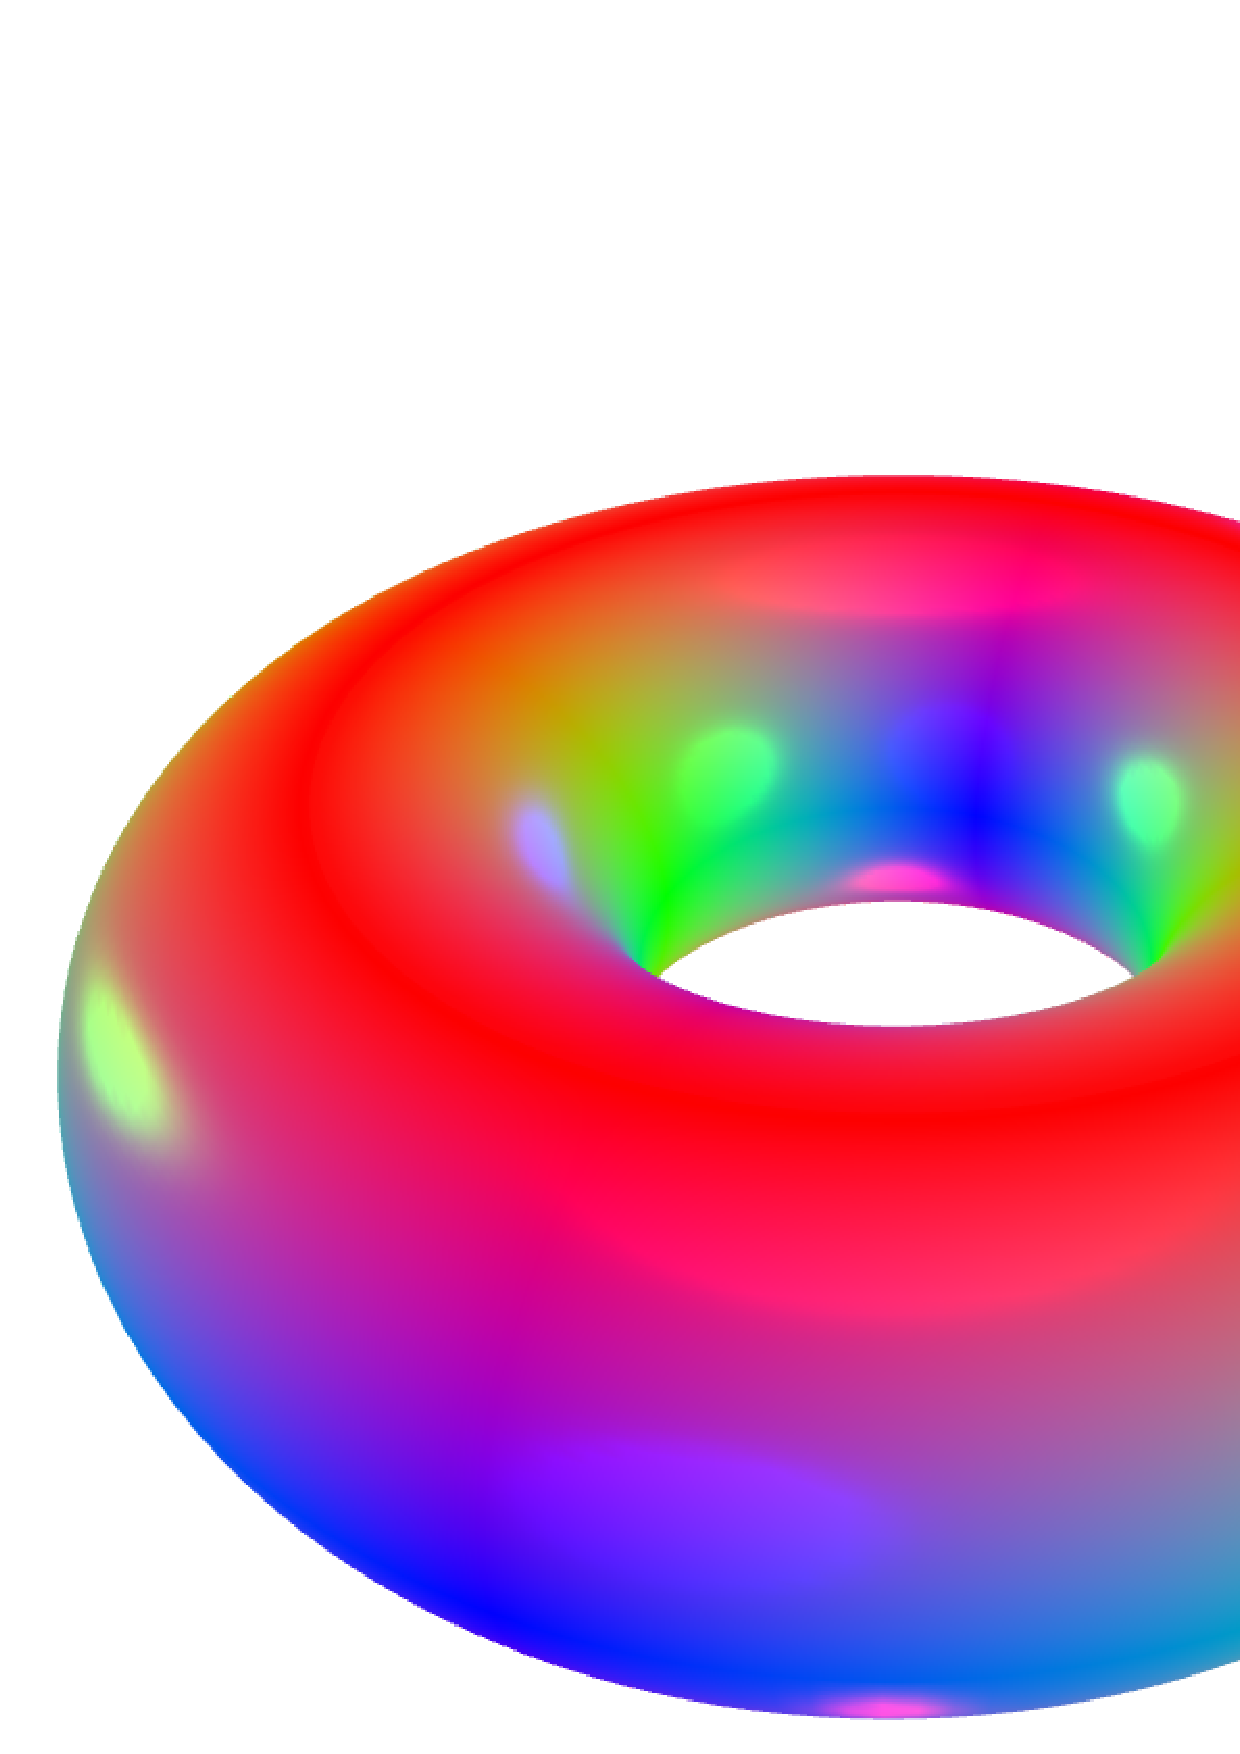
\includegraphics[height=0.22\textheight]{images/graphs/donut.png}
\subsection{Schnecke}
\begin{tabular}[b]{|l|c|}
\hline
\rowcolor[gray]{0.5}
Art &  3D Parametrisch \\
\rowcolor[gray]{1}
\(x(u,v)\) & \((\sin(u)+\frac{v}{2 \cdot \pi}) \cdot \sin(v) \cdot v\) \\
\rowcolor[gray]{0.5}
\(y(u,v)\) & \((\sin(u)+\frac{v}{2 \cdot \pi}) \cdot \cos(v) \cdot v\) \\
\rowcolor[gray]{1}
\(z(u,v)\) & \(\cos(u) \cdot v\) \\
\rowcolor[gray]{0.5}
Min \(u\) & \(-\pi\) \\
\rowcolor[gray]{1}
Max \(u\) & \(\pi\) \\
\rowcolor[gray]{0.5}
Step \(u\) & \(\frac{\pi}{50}\) \\
\rowcolor[gray]{1}
Min \(v\) & \(0\) \\
\rowcolor[gray]{0.5}
Max \(v\) & \(30\) \\
\rowcolor[gray]{1}
Step \(v\) &\(0.05\) \\
\hline
\end{tabular}
\includegraphics[height=0.22\textheight]{images/graphs/schnecke.png}
\subsection{Kleinsche Flasche}
\begin{tabular}[b]{|l|c|}
\hline
\rowcolor[gray]{0.5}
Art &  3D Parametrisch \\
\rowcolor[gray]{1}
\(x(u,v)\) & \(3 \cdot \cos(u) \cdot (1+\sin(u))-(2-\cos(u)) \cdot \cos(v)\) \\
\rowcolor[gray]{0.5}
\(y(u,v)\) & \(8 \cdot \sin(u)\) \\
\rowcolor[gray]{1}
\(z(u,v)\) & \(\sin(v) \cdot(2-\cos(u))\) \\
\rowcolor[gray]{0.5}
Min \(u\) & \(-\pi\) \\
\rowcolor[gray]{1}
Max \(u\) & \(\pi\) \\
\rowcolor[gray]{0.5}
Step \(u\) & \(\frac{\pi}{100}\) \\
\rowcolor[gray]{1}
Min \(v\) & \(-\pi\) \\
\rowcolor[gray]{0.5}
Max \(v\) & \(\pi\) \\
\rowcolor[gray]{1}
Step \(v\) &\(\frac{\pi}{100}\) \\
\hline
\end{tabular}
\includegraphics[height=0.22\textheight]{images/graphs/kleinsche_flasche.png}
\newpage
\section{Dateien}
\subsection{Log}
\label{chp:Log}
Zus"atzlich zu der Programm- und Konsolenausgabe gibt es noch zwei weitere Logdateien. Diese befinden sich im Programmordner, genauer gesagt dort im Ordner log. Dort gibt es die Dateien logfile-user.txt und logfile-debug.txt. Wie der Name schon sagt ist das Erste als Einblick f"ur den Benutzer gedacht und das Zweite f"ur den Entwickler. Bei Problemen mit dem Programm sollte daher auch immer das Entwickler-Log mitgeschickt werden.
\subsection{Optionen}
Die Programmoptionen befinden sich an der Stelle Anwendungsdaten/.graphs/options.txt. Der Pfad kann je nach System etwas abweichen. Sollte dieser Ordner, bzw. die Datei nicht existieren oder Fehler enthalten, so wird der Ordner automatisch erstellt, bzw. eine Datei mit den Standardeinstellungen erstellt.
\subsection{Cubemaps}
\begin{wrapfigure}{r}{3cm}
\includegraphics[height=0.10\textheight]{images/cube.png} 
\caption{Cubemap}
\end{wrapfigure}
Das Programm kann mit jeder Cubemap umgehen, wenn sie in der Form vorliegt, dass sich 6 von 0 bis 5 durchnummerierte und passend gedrehte Bilder in einem Ordner befinden. Der Pfad der zu benutzenden Cubemap l"asst sich im Optionenfenster w"ahlen.
\subsection{Graph}
Das Standardformat f"ur Projekte. Es ist ein Zip-Archiv, das die Daten in Form von Textdateien im Unicode-Format enth"alt.
\subsection{Off}
Ein Format, dass sich daf"ur eignet um die Graphen f"ur andere Programme zu exportieren, die Sie dann rendern k"onnen. Dies kann sinnvoll sein, wenn einem die Qualit"at der Bilder nicht ausreicht, bzw Rendereinstellungen erw"unscht sind, die vom Programm nicht unterst"utzt werden. Beispielsweise k"onnen mit dem freien Programm Blender sehr sch"one Bilder erzeugt werden.
\subsection{Jar}
Die jar-Dateien sind die Programme, die von der jvm (Java Virtual Machine) interpretiert werden.
\newpage
\section{H"aufige Probleme}
\subsection{Programm startet nicht}
\begin{tabular}[b]{|lp{7cm}|lp{7cm}|}
\hline
Ursache & L"osung \\
\hline
Java-Version ist zu alt & Installieren Sie Java mit Version >= 6.\\
\hline
\end{tabular}
\subsection{Kein 3D-Fenster}
\begin{tabular}[b]{|lp{7cm}|lp{7cm}|}
\hline
Ursache & L"osung \\
\hline
Grafiktreiber unterst"utzt OpenGl nicht & Installieren Sie den neuesten Treiber des Herstellers und "uberpr"ufen Sie, ob OpenGl unterst"utzt wird.\\
\hline
LWJGL ist unter Linux nicht installiert oder zu alt & Installieren Sie mindestens Version 2.8.1 von LWJGL auf ihrem Linux System.\\
\hline
\end{tabular}
\end{document}
